\subsection{Aufbau}
Um den normalen und annormalen Zemman-Effekt zu messen, werden die Spektrallinien einer Cadmium-Lampe aufgenommen.
Von Bedeutung sind dabei die Spektrallinien der Wellenlängen $\SI{643.8}{\nano\meter}$ (blau), welche beim Übergang ${}^1P_1\leftrightarrow{}^1D_2$ entsteht, und
die Wellenlänge $\SI{480}{nm}$ (rot), welche beim Übergang ${}^1S_1\leftrightarrow{}^3P_1$ entsteht.
Mit der Wellenlänge im blauen Bereich kann der annormale Zeeman-Effekt beobachtet werden.
Der normale Zeeman-Effekt kann mit der Wellenlänge im roten Bereich betrachtet werden.\\
%
Um die Zeeman-Aufspaltung zu erzeugen wird die Cadmium-Lampe (Cd-Lampe) zwischen zwei Polschuhe eines Elektromagneten gebracht.
Die Emissionslinien der Cd-Lampe werden transversal zum Magnetfeld kollimiert.
Unter Verwendung eines Geradsichtprismas werden die Wellenlängen räumlich separiert.
Mithilfe eines Spaltes kann die zu untersuchende Spektrallinie von den andere Wellenlänge separiert werden.
Durch einen Polarisationsfilter kann die Spektrallinie auf $\pi$- oder $\sigma$- Übergänge untersucht werden.
Die transversale Betrachtung sorgt dafür, dass sowohl $\pi$- als auch $\sigma$-Licht linear polarisiert erscheint.
Entsprechend lässt der Polarisationsfilter lässt je nach Einstellung nur $\pi$- oder $\sigma$-Licht durch.
Bei der senkrechten Stellung zu $\vec{B}$ fällt das $\sigma$-Licht hindurch, bei paralleler Stellung zu $\vec{B}$ fällt das $\pi$-Licht hindurch.
%Der Polarisationsfilter lässt nur linear polarisiertes Licht durch, ist jedoch drehbar.
%Die Messung ist transversal.
%Das bedeutet, dass linear polarisiertes Licht ($\pi$) in jeder Stellung des Polarisationsfilters durchfällt, zirkular polarisiertes ($\sigma$) fällt jedoch nur bei einer senkrechten Ausrichtung des Polarisationsfilters durch.
Die nachgeschaltete Lummer-Gehrcke-Platte erzeugt ein Interferenzmuster, welches von einer Digitalkamera aufgezeichnet wird.
Mithilfe der erzeugten Interferenz kann ein sehr hohes Auflösungsvermögen erzielt werden.
Trifft monoenergetisches Licht auf die Lummer-Gehrcke-Platte so entstehen Interferenzstreifen, welche genau einen Gangunterschied von der eingestrahlten Wellenlänge besitzen.
Bei eingeschaltetem Magnetfeld kommt es zur Aufspaltung der Spektrallinien.
Die maximale Differenz der eingestrahlten Wellenlängen, damit sich die Wellen nicht überlagern, ist durch das Dispersionsgebiet $\Delta \lambda_D$ gegeben:
\begin{align}
	\Delta \lambda_D =\frac{\lambda^2}{2d}\sqrt{\frac{1}{n^2-1}}.
	\label{eqn:dispersionsgebiet}
\end{align}
$d$ ist dabei die Dicke der Lummer-Gehrcke-Platte und $n$ der Brechungsindex für die jeweilige Wellenlänge.
Die Wellenlängenänderung ist dabei gegeben als:
\begin{align}
  \delta \lambda = \frac{1}{2}\frac{\delta s}{\Delta s}\cdot \Delta\lambda_D.
	\label{eqn:wellenlänge}
\end{align}
Die Lummer-Gehrcke-Platte der Länge $L$ besitzt zudem ein Auflösungsvermögen von:
\begin{align}
 A=\frac{\lambda}{\Delta\lambda}=\frac{L}{\lambda}(n^2-1).
 \label{eqn:auflösung}
\end{align}
\FloatBarrier


\subsection{Durchführung}
Zunächst wird die Vermessung des Elektromagneten, mittels Messung des B-Feldes in Abhängigkeit vom Feldstrom, vorgenommen.
Der Strom wird erhöht und anschließend verringert.
Auf diese Weise lässt sich eine Hysteresekurve messen.\\
Anschließend wird die Cd-Lampe eingeschaltet und die Linsen werden justiert.
%Unter Verwendung der Linsen können bestimmt Spektrallinien betrachtet werden.
Desweiteren wird ein Polarisator in den Strahlengang gebracht.
Dieser erlaubt, einzelne Strahlen mit bestimmter Polarisation zu betrachten.
So werden $\pi$- ($\Delta m = 0$) und $\sigma$- ($\Delta m = \pm 1$) Übergänge getrennt.
Eine am Ende des Strahlengangs angebrachte Digitalkamera kann die Interferenzmuster der Lummer-Gehrcke-Platte aufnehmen und abspeichern.\\
%
Die erste Messung wird mit dem $\sigma$-Übergang der roten Linie durchgeführt (normaler Zeeman-Effekt).
Durch langsames Erhöhen des Magnetfeldes kann darauf geachtet werden, dass sich die Linien klar aufteilen, die Wellenlängendifferenz jedoch noch nicht größer als das Dispersionsgebiet wird.
Die Interferenzmuster werden mit der Kamera aufgenommen.
Dabei wird zunächst jeweils ein Bild der Interferenzmuster mit $B=0$ aufgenommen, dann die Bilder mit $B≠0$.
Für die rote Linie wird ein Bild des $\sigma$-Übergangs mit $B≠0$ gespeichert.
Für die blaue Linie werden ein Bild des $\sigma$-Übergangs und ein Bild des $\pi$-Übergangs gemacht.
Im folgenden wird aus den Bildern mit $B=0$ der Wert des Abstands der Interferenzmuster $\Delta s$ bestimmt (\ref{fig:auslesen}).
Aus den Bildern mit $B≠0$ wird die Weite der Aufspaltung der Interferenzmuster $\delta s$ entnommen.
\begin{figure}[h!]
  \centering
  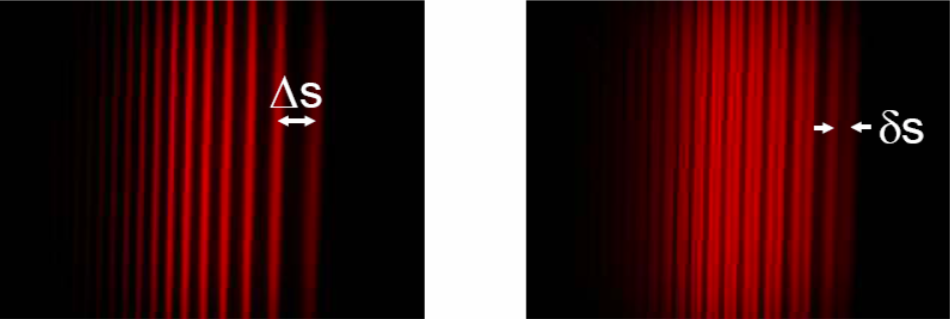
\includegraphics[width=\textwidth]{auslesen.png}
  \caption{Darstellung der Werte $\Delta s$ und $\delta s$ \cite{1}}
  \label{fig:auslesen}
\end{figure}

%Die Messung wird für die $\pi$- und $\sigma$- Übergänge des blauen Lichtes analog durchgeführt.
\FloatBarrier
